\chapter{Project Management}
\section{Organization}
The work for this project has been done by me, but also with the help and supervision of Prof. Stefan Keller, and with the help of Nicola Jordan of the HSR Software Institute.
The source code is open in GitLab with an MIT license (for now).\\
The source code can be found here: \href{https://gitlab.com/labiangashi/python-wfs-server}{gitlab.com/labiangashi/python-wfs-server}
\section{Planning \& Coordination}
Meetings have been held regularly every week in Zurich or in the HSR institute to discuss the week's achievements, obstacles and plans for the next week. An agile software development process was used and each sprint lasted 1 to 2 weeks.
The project started on 15 Sep 2019 and lasted around 8 sprints.\\
\newline
The initial sprints were mostly information gathering, defining the functional requirements, the languages to be used, tools, libraries, software architecture \& design etc.\\
After those decisions were made and the couple of initial sprints were finished, then began the phase of developing the application, this phase was preliminary finished in about 4 sprints.\\
After this phase, for the last two sprints, began the phase of testing (unit testing, load testing, integration testing etc) and making sure everything is fine before dockerizing the application.\\
The last phase was the phase of documenting the project.
\section{Workflow}
The application was coded using the \href{https://www.jetbrains.com/pycharm/}{PyCharm} IDE, which is a Python IDE for professional Python developers, it offers a lot of features and is all around a great environment for developing in Python.\\
As mentioned above in the \hyperref[sec:GitLab]{Implementation} chapter, the code repository and CI/CD tools for this application was \href{https://gitlab.com/}{GitLab}.\\
Here are some of the graphs that were taken from GitLab for this project:
\begin{figure}[H]
	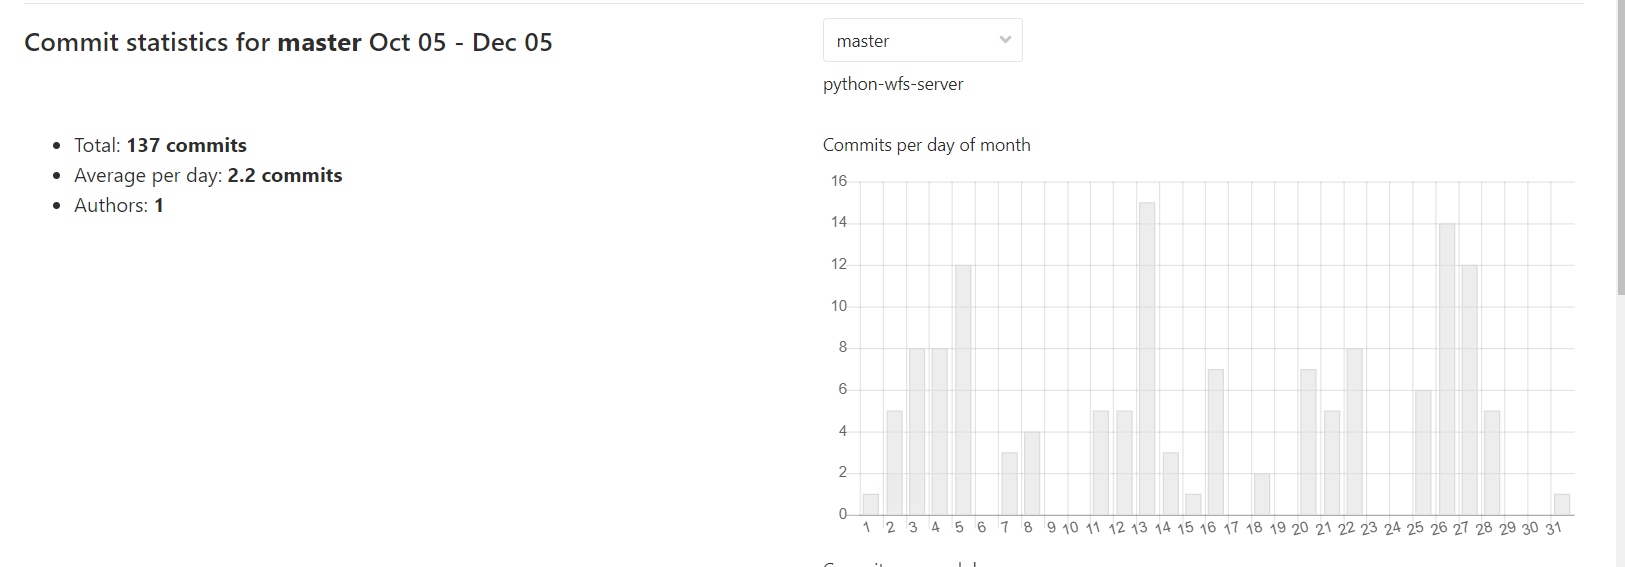
\includegraphics[width=\linewidth]{./Images/Appendices/commits_graph.png}
	\caption{Information about GitLab commits}
\end{figure}
\begin{figure}[H]
	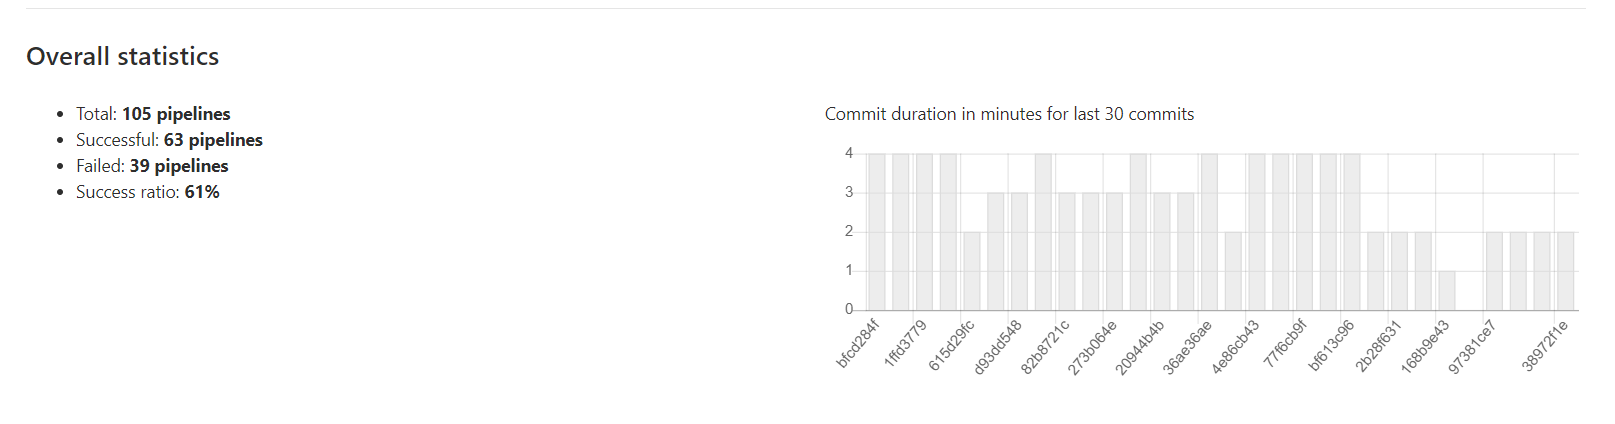
\includegraphics[width=\linewidth]{./Images/Appendices/pipelines_graph.png}
	\caption{Information about CI/CD pipelines}
\end{figure}